%%%%%%%%%%%%%%%%%%%%%%%%%%%%% Define Article %%%%%%%%%%%%%%%%%%%%%%%%%%%%%%%%%%
\documentclass[twocolumn]{article}
%%%%%%%%%%%%%%%%%%%%%%%%%%%%%%%%%%%%%%%%%%%%%%%%%%%%%%%%%%%%%%%%%%%%%%%%%%%%%%%

%%%%%%%%%%%%%%%%%%%%%%%%%%%%% Using Packages %%%%%%%%%%%%%%%%%%%%%%%%%%%%%%%%%%
\usepackage{geometry}
\usepackage{graphicx}
\usepackage{amssymb}
\usepackage{amsmath}
\usepackage{amsthm}
\usepackage{empheq}
\usepackage{mdframed}
\usepackage{booktabs}
\usepackage{lipsum}
\usepackage{graphicx}
\usepackage{color}
\usepackage{psfrag}
\usepackage{pgfplots}
\usepackage{bm}
%%%%%%%%%%%%%%%%%%%%%%%%%%%%%%%%%%%%%%%%%%%%%%%%%%%%%%%%%%%%%%%%%%%%%%%%%%%%%%%

\usepackage[brazil]{babel}
\usepackage{babelbib}
\usepackage{url}
\usepackage{titlesec}
\usepackage{hyperref}
\usepackage{float}
\usepackage[nonumberlist,acronym,automake=immediate]{glossaries}

\titleformat{\section}[runin]{\normalfont\large\bfseries}{}{0pt}{}
\titleformat{\subsection}[runin]{\normalfont\normalsize\bfseries}{}{0pt}{}
\titleformat{\subsubsection}[runin]{\normalfont\small\bfseries}{}{0pt}{}



\newcounter{anexo}
\newenvironment{anexo}[1]
    {
    \titleformat{\section}{\normalfont\large\bfseries}{}{0pt}{}
        \refstepcounter{anexo}
        \newpage
        \section{Anexo \theanexo: #1}

    }
    {
    }
%%%% Glossary %%%%%%%%%%%%%%%%%%%%%%%%

\makeglossaries
\newacronym{mccrm}{MCCRM}{Minimização de Arrependimento Contrafactual de Monte Carlo}
\newacronym{crm}{CRM}{Minimização de Arrependimento Contrafactual}
\newacronym{ia}{IA}{Inteligência Artificial}
\newacronym{gto}{GTO}{Ótimo Em Teoria dos Jogos}

\newglossaryentry{flush}{
    name=flush,
    description={Um jogo em poker em que um jogador possui cinco cartas do mesmo naipe}
}

\newglossaryentry{arrep}{
    name=arrependimento,
    description={O quanto um agente preferiria ter tomado uma decisão à decisão real dele}
}

\newglossaryentry{esnash} {
    name={estratégia de Nash},
    description={Uma estratégia ótima em um equillíbrio de Nash. Desvios de uma estratégia de Nash, não podem melhorar a performance
    de um agente},
    plural={estratégias de Nash}
}

\newglossaryentry{estrategia} {
    name={estratégia},
    description={
        Uma descrição de qual ação deve ser tomada em cada estado de um jogo
    }
}

\newglossaryentry{no} {
    name={nó},
    description={
        Uma dos possíveis estados de jogo em uma árvore de decisão
    }
}

\newglossaryentry{nof} {
    name={nó folha},
    description={
        Um nó no fim de uma árvore de decisão, que não possui arestas de saída
    }
}


\newglossaryentry{equidade} {
    name={equidade},
    description={
        A sua probabilidade de ganhar uma mão. Uma de suas variações é a equidade de fold, que representa
        a probabilidade do seu adversário foldar com a sua aposta
    }
}

\newglossaryentry{icm} {
    name={independent chip modelling},
    description={Conceito de que suas fichas no poker possuem valores diferentes dependendo do momento do jogo em
    que você se encontra. Aplicado principalmente em torneios de poker}
}

\newglossaryentry{odds} {
    name={odds},
    description={Quanto de equidade você precisa para, com a aposta atual na mesa, valer a pena você entrar na mão}
}

\newglossaryentry{evalue} {
    name={valor esperado},
    description={Valor esperado ao se fazer uma jogada. Leva em conta a equidade das cartas em mão e no jogo}
}

\newglossaryentry{arvore} {
    name={árvore de decisões},
    description={Representação de um jogo como uma árvore em que cada nó é um estado do jogo, e cada aresta
    representa uma decisão que pode ser tomada pelos jogadores}
}

\newglossaryentry{valor} {
    name={valor},
    description={O valor de um nó na árvore de jogadas}
}

\newglossaryentry{nlh} {
    name={no limit holdem},
    description={
        Variante do poker em que dois ou mais jogadores jogam com duas cartas na mão
        e cinco cartas na mesa, e que os jogadores não possuem limites de aposta
    }
}

\newglossaryentry{lh} {
    name={limit holdem},
    description={
        Variante do poker em que dois ou mais jogadores jogam com duas cartas na mão
        e cinco cartas na mesa, e que os jogadores possuem limites de aposta determinados
        pelo tamanho do \emph{pot} no momento
    }
}

\newglossaryentry{pot} {
    name={pot},
    description={
        Quantidade de apostas que está em jogo até o momento no poker
    }
}

\glsaddall
%%%%%%%%%%%%%%%%%%%%%%%%%% Page Setting %%%%%%%%%%%%%%%%%%%%%%%%%%%%%%%%%%%%%%%
\geometry{a4paper}
\pagenumbering{roman}


%%%%%%%%%%%%%%%%%%%%%%%%%% Define an orangebox command %%%%%%%%%%%%%%%%%%%%%%%%
\newcommand\orangebox[1]{\fcolorbox{ocre}{mygray}{\hspace{1em}#1\hspace{1em}}}
%%%%%%%%%%%%%%%%%%%%%%%%%%%%%%%%%%%%%%%%%%%%%%%%%%%%%%%%%%%%%%%%%%%%%%%%%%%%%%%

%%%%%%%%%%%%%%%%%%%%%%%%%%%% English Environments %%%%%%%%%%%%%%%%%%%%%%%%%%%%%
\newtheoremstyle{mytheoremstyle}{3pt}{3pt}{\normalfont}{0cm}{\rmfamily\bfseries}{}{1em}{{\color{black}\thmname{#1}~\thmnumber{#2}}\thmnote{,--,#3}}
\newtheoremstyle{myproblemstyle}{3pt}{3pt}{\normalfont}{0cm}{\rmfamily\bfseries}{}{1em}{{\color{black}\thmname{#1}~\thmnumber{#2}}\thmnote{,--,#3}}
\theoremstyle{mytheoremstyle}
\newmdtheoremenv[linewidth=1pt,backgroundcolor=shallowGreen,linecolor=deepGreen,leftmargin=0pt,innerleftmargin=20pt,innerrightmargin=20pt,]{theorem}{Theorem}[section]
\theoremstyle{mytheoremstyle}
\newmdtheoremenv[linewidth=1pt,backgroundcolor=shallowBlue,linecolor=deepBlue,leftmargin=0pt,innerleftmargin=20pt,innerrightmargin=20pt,]{definition}{Definition}[section]
\theoremstyle{myproblemstyle}
\newmdtheoremenv[linecolor=black,leftmargin=0pt,innerleftmargin=10pt,innerrightmargin=10pt,]{problem}{Problem}[section]
%%%%%%%%%%%%%%%%%%%%%%%%%%%%%%%%%%%%%%%%%%%%%%%%%%%%%%%%%%%%%%%%%%%%%%%%%%%%%%%

%%%%%%%%%%%%%%%%%%%%%%%%%%%%%%% Plotting Settings %%%%%%%%%%%%%%%%%%%%%%%%%%%%%
\usepgfplotslibrary{colorbrewer}
\pgfplotsset{width=8cm,compat=1.9}
%%%%%%%%%%%%%%%%%%%%%%%%%%%%%%%%%%%%%%%%%%%%%%%%%%%%%%%%%%%%%%%%%%%%%%%%%%%%%%%

%%%%%%%%%%%%%%%%%%%%%%%%%%%%%%% Title & Author %%%%%%%%%%%%%%%%%%%%%%%%%%%%%%%%
\title{Inteligência Artificial de Poker No Limit Holdem\\Pluribus}
\author{Pedro Tavares de Carvalho}
%%%%%%%%%%%%%%%%%%%%%%%%%%%%%%%%%%%%%%%%%%%%%%%%%%%%%%%%%%%%%%%%%%%%%%%%%%%%%%%

\begin{document}
        \maketitle

        \thispagestyle{empty}
        \abstract{
            Nesse projeto, iremos discutir a inteligência artificial de poker chamada \emph{Pluribus}~\cite{brown2019superhuman},
            seus detalhes de implementação e design, além de seus impactos na sociedade e no futuro de \acrfull{ia} em jogos.
            Abordaremos o poker como um jogo em teoria de jogos, seu processo de modelagem e os desafios
            existentes ao se tratar de um jogo como o poker em uma inteligência artificial.
            }


    \section{Introdução} % (fold)
    \label{sec:Introdução}
        O poker é um dos jogos mais jogados do mundo. Com regras simples de se entender, porém
        difíceis de se dominar, o poker atende jogadores casuais e aficionados da mesma forma.

        Apesar de sua popularidade, a revolução das inteligências artificiais, que inclui damas~\cite{5392560}, xadrez~\cite{CAMPBELL200257}
        e mais recentemente GO~\cite{Silver2016}, atingiu diversos outros jogos antes do poker. Muito disso se deve à
        dificuldade de se modelar uma \gls{estrategia} ótima em poker.

        A história da inteligência artifical no poker é longa, incluindo diversas \glspl{estrategia}, dentre elas algoritmos genéticos~\cite{4219032} e
        aprendizado profundo~\cite{DBLP:journals/corr/MoravcikSBLMBDW17}. Uma versão mais simplificada do poker, o Limit Texas Holdem, onde os jogadores possuem
        limites em quanto eles podem apostar, já foi fechada matematicamente~\cite{bowling2015heads}.

        Iremos explorar no que o Pluribus difere das \glspl{estrategia} empregadas até o momento, e o motivo dessas \glspl{estrategia} serem menos eficientes
        e menos efetivas do que as novas, modelando o poker matematicamente e observando os detalhes que fizeram o Pluribus quebrar a barreira
        do poker sem limites com 6 jogadores.

    % section Introdução (end)

    \section{Modelagem do Poker em Teoria de Jogos } % (fold)
    \label{sec:Modelagem do Poker em Teoria de Jogos }
        O poker pode ser modelado em teoria de jogos como um jogo:

        \begin{description}
            \item[De informação incompleta] Os agentes do jogo não possuem acesso a quais cartas os seus adversários estão na mão, ou seja,
                com as informações que ele tem no momento, não é possível determinar com certeza em qual estado de jogo o mesmo está.

            \item[Adversarial] Os agentes jogam com o objetivo de ganhar, sem colaborar entre si.

            \item[Soma zero] Quando um dos agentes joga, uma combinação dos outros perde, tornando o valor total existente no jogo fixo.

            \item[Estocástico] Ações dentro do poker podem produzir estados diferentes, e, consequentemente, valores diferentes.
        \end{description}

        Em geral, o poker difere de jogos como xadrez e GO por alguns motivos, incluindo o fato de ele ser um jogo de informação incompleta
        e estocástico, e pelo fato de o mesmo ser jogado com mais de dois jogadores, o que torna a \gls{estrategia} e a busca dentro da \gls{arvore}
        mais complexa do que um minimax simples.

        \subsection{Equilíbrio de Nash e Poker GTO} % (fold)
        \label{ssub:Equilíbrio de Nash e Poker GTO}
            O poker, quando jogado por pessoas reais, é dividido em duas vertentes principais, a vertente exploitativa, que tenta se aproveitar
            de erros na \gls{estrategia} do seu adversário, e o poker \acrfull{gto}, que tenta maximizar matematicamente a \gls{estrategia},
            tentando atingir um Equilíbrio de Nash~\cite{nash1950equilibrium}.

            Em poker sem limites, não existe uma \gls{esnash} fechada, o que é feito são tentativas de aproximação dessa \gls{estrategia},
            no caso do poker humano, com conceitos como \gls{evalue},
            \emph{\gls{icm}}~\cite{gilbert2009independent}, \gls{equidade},
            \gls{odds}, entre outros
            que ajudam a aproximar a melhor ação em cada momento. Já em inteligências artificiais, a técnica mais usada é a de \acrfull{crm}, que atualiza a \gls{arvore} tentando diminuir a quantidade de decisões erradas.


        % subsubsection Equilíbrio de Nash e Poker GTO (end)
    % section Modelagem do Poker em Teoria de Jogos  (end)

    \section{O Pluribus por alto} % (fold)
    \label{sec:O Pluribus por alto}
        O Pluribus é composto de três peças principais, abstração de informação, o croqui de \gls{estrategia} construído por minimização de \gls{arrep},
        e o algoritmo de busca em tempo real que cria \gls{estrategia} em \glspl{no} não antes explorados.

        A \gls{estrategia} do Pluribus foi construída, principalmente, por jogos com versões de si mesmo. Utilizando versões antigas
        da sua \gls{estrategia} como adversários, ele emula jogos e melhora a sua performance.
        Esse método é muito utilizado em inteligências
        artificiais, incluindo o xadrez~\cite{DBLP:journals/corr/abs-1712-01815} e GO~\cite{Silver2016}. Com esses jogos, o Pluribus desenvolve uma \gls{estrategia}
        base, que é utilizada e atualizada no momento da busca em tempo real, quando o agente está realmente jogando.
    % section O Pluribus por alto (end)

    \section{Abstrações de Informação } % (fold)
    \label{sec:Simplificação de Informação }
        Para simplificar a busca e melhorar a \gls{estrategia} da \acrshort{ia}, o Pluribus aplica técnicas de simplificação de informação, tanto a nível de apostas
        possíveis quanto a nível de valor de mão.

        \subsection{Abstração de Apostas} % (fold)
        \label{sub:Simplificação de Apostas}

            A simplificação de apostas age tanto no espaço de apostas consideradas pelo agente em sua jogada quanto em apostas de adversários. O processo
            é uma discretização das apostas, transformando valores específicos de apostas em um conjunto específico de apostas possíveis.

        % subsection Simplificação de Apostas (end)

        \subsection{Abstração de Mãos} % (fold)
        \label{sub:Simplificação de Mãos}
            Esse processo diminui o espaço de mãos possíveis dentro de um jogo de poker. A idéia é que mão de valores similares, como um \emph{flush}
            com carta alta em 10 e um \emph{\gls{flush}} com carta alta em 9, serão agrupadas em um mesmo conjunto, e ações similares (se não idênticas) serão
            tomadas em situações que surgem com essas mãos.

            Isso não é uma regra, e dependendo da especificidade da situação, a abstração pode ser desconsiderada, e as mãos podem ser tratadas como
            diferentes pela \gls{estrategia}.

        % subsection Simplificação de Mãos (end)

    % section Simplificação de Informação  (end)

    \section{Minização de arrependimento contrafactual de Monte Carlo} % (fold)
    \label{sec:Minização de arrependimento contrafactual de Monte Carlo}
        Para a construção da \gls{estrategia} base, é utilizada uma técnica chamada de \acrfull{mccrm}~\cite{NIPS2009_00411460,brown2019solving}.

        Essa técnica consiste na simulação de jogos da \acrshort{ia} contra si mesma, e da revisão das decisões tomadas no jogo completo a fim de minimizar o "\gls{arrep}"
        do agente, ou seja, aumentando a probabilidade de decisões boas e diminuindo a de decisões ruins.

        Diferente da \acrshort{crm} normal, em que a cada geração da \gls{estrategia} a \gls{arvore} completa é atualizada, o \acrshort{mccrm} simula somente um jogo\footnote{Um jogo é uma descida
        completa na \gls{arvore}, até se chegar em um \gls{nof}.} de todos os possíveis, e atualiza as decisões que são geradas nesse jogo somente.

    % section Minização de arrependimento contrafactual de Monte Carlo (end)

    \section{Busca em jogos de informação incompleta} % (fold)
    \label{sec:Busca em Jogos de informação incompleta}

        Diferente de jogos de infomação completa, como xadrez e GO, em que você consegue ter certeza do estado em que você está e da \gls{estrategia} do seu adversário,
        busca em ambientes de informação incompleta não conseguem se basear apenas na avaliação de um estado na \gls{esnash}, ao menos não de um estado não-folha.

        Isso acontece pois a avaliação assume que o adversário não usará uma \gls{estrategia} diferente no futuro, ou seja, continuará utilizando uma \gls{esnash}
        ótima, e portanto tomará as mesmas decisões. Isso pode ser visto na figura \ref{fig:rps}, onde uma busca em um jogo de pedra papel ou tesoura
        causa uma \gls{estrategia} que não implica em otimalidade.

        Por exemplo, se tivéssemos um algoritmo guloso, uma busca poderia sempre resultar em \emph{pedra}
        como ação, o que faria com que se um adversário racional mudasse sua \gls{estrategia}, ele pudesse explorar os nossos vieses.


        \begin{figure}
            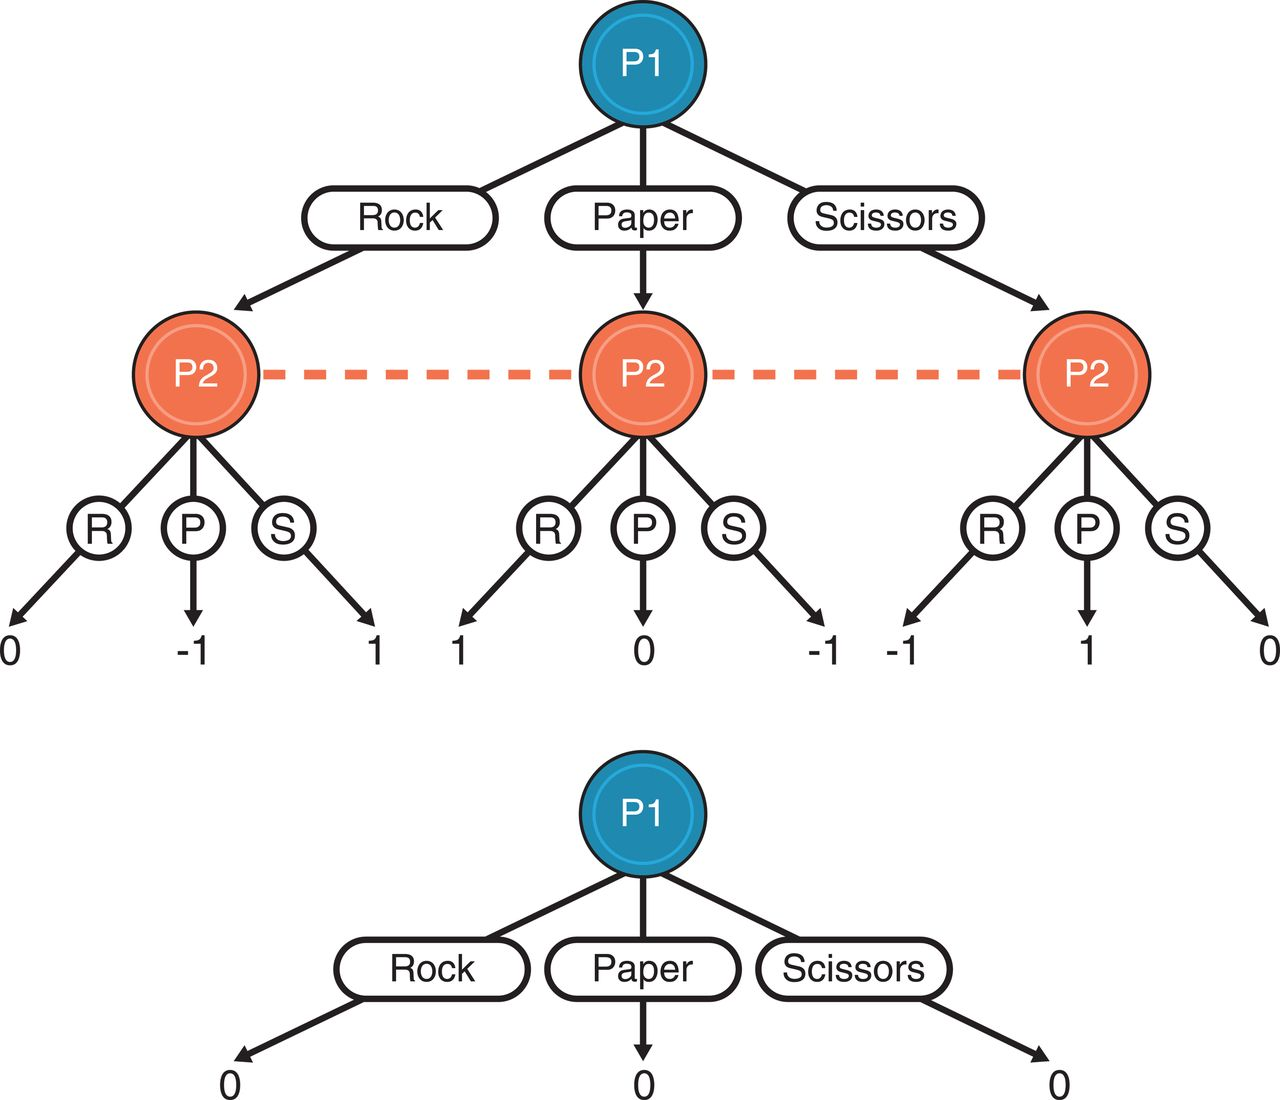
\includegraphics[width=0.48\textwidth]{./rps.jpeg}
            \caption{Avaliação e busca em um jogo de pedra papel ou tesoura. Primeiro se vê a descida das decisões e valores possíveis
            na árvore, depois se vê a avaliação de cada decisão em uma \gls{esnash}.}
            \label{fig:rps}
        \end{figure}

        Para contornar esse problema, o Pluribus aplica uma técnica de pesquisa com profundidade limitada~\cite{brown2018depth} em que diferentes \glspl{estrategia}
        adversárias são emuladas e avaliadas, observando o valor em todas elas. Para o Plúribus, foram utilizadas 4 \glspl{estrategia} diferentes, sendo essas
        vieses construídos a partir da \emph{blueprint} de \gls{estrategia} gerada com o \hyperref[sec:Minização de arrependimento contrafactual de Monte Carlo]{\acrshort{mccrm}}.

    % section Busca em Jogos de informação incompleta (end)

    \section{Impactos do Pluribus} % (fold)
    \label{sec:Impactos do Pluribus}

    O Pluribus, apesar da falta de visibilidade, representa uma nova revolução dentro do mundo de
    \acrlong{ia} para jogos. Nenhum projeto até o momento havia conseguido boas emulações de
    \glspl{esnash} em jogos de informação incompleta com mais de dois jogadores.

    Essa modelagem de sistema se aplica em diversas situações da vida real, incluindo negociações de vendas,
    interações diplomáticas e diversas outras situações em que várias pessoas disputam pelos mesmos
    recursos.

    Dentro do poker, o Pluribus representa um possível problema para o grande cenário online de poker.
    Esse cenário possui diversos profissionais do jogo, e possui campeonatos de milhões
    de dólares~\cite{scoop}.

    Alguns provedores de poker online já possuem ações contra jogadores automáticos de poker~\cite{botdec},
    porém as técnicas de detecção não são muito claras. Assim como no xadrez online~\cite{bilen2021online,barnes2015limits},
    essas técnicas de detecção se desenvolverão mais à medida que mais bots forem desenvolvidos e forem mais
    acessíveis.

    % section Impactos do Pluribus (end)

    \onecolumn
    \clearpage
    \printglossary
    \printglossary[type=\acronymtype]
    \nocite{*}
    \bibliographystyle{bababbrv}
    \bibliography{referencias}

    \begin{anexo}{Mãos de poker}
        \begin{figure}[H]
            \begin{center}
                \includegraphics[height=0.9\textheight]{Ranking-de-Mãos-Completo.png}
            \end{center}
            \caption{Ranking de mãos de poker}
            \label{fig:ranking}
        \end{figure}

    \end{anexo}


\end{document}
